%-*-latex-*-
\sectionthree{Heapify-up}
\begin{python0}
from solutions import *; clear()
\end{python0}

The following two operations are the basic tools for min- and maxheaps.

Look at this:

%-*-latex-*-

\begin{center}
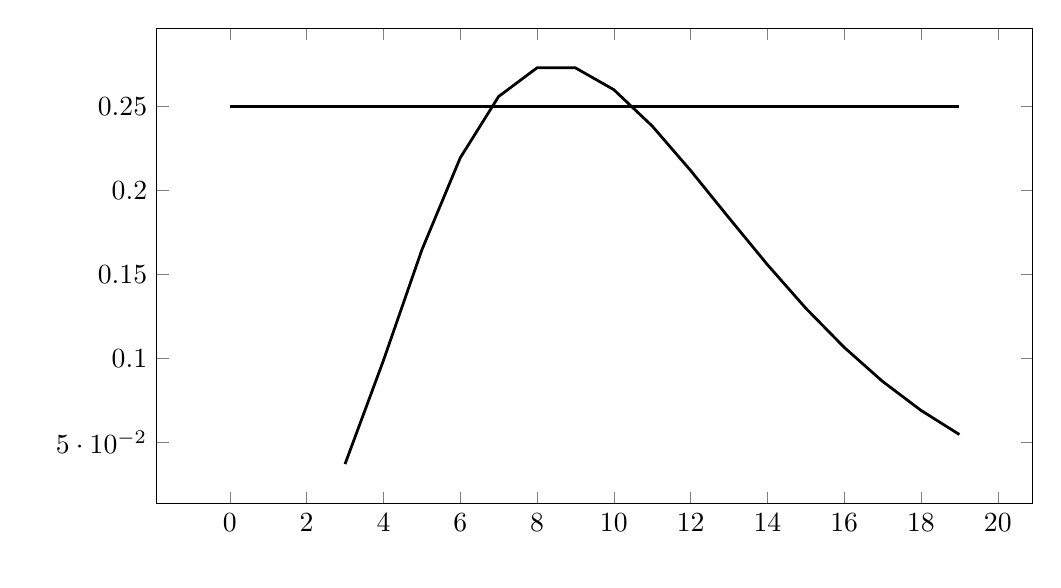
\begin{tikzpicture}[line width=1]
\begin{axis}[width=5in, height=3in,
             scatter/classes={a={mark=*,draw=black}},
             xlabel={\mbox{}},
             xlabel style={name=xlabel}, 
             ylabel={\mbox{}}, 
             legend style={
                at={(xlabel.south)},
                yshift=-1ex,
                anchor=north,
                legend cell align=left,
                },
        ]
]
\addplot[draw=black, line width=1] coordinates {(3, 0.03703703703703703)
(4, 0.0987654320987654)
(5, 0.16460905349794233)
(6, 0.21947873799725642)
(7, 0.2560585276634658)
(8, 0.2731290961743635)
(9, 0.2731290961743635)
(10, 0.26012294873748903)
(11, 0.23844603634269826)
(12, 0.2119520323046207)
(13, 0.18369176133067125)
(14, 0.15585967628056951)
(15, 0.12988306356714127)
(16, 0.10657071882432105)
(17, 0.08627153428635512)
(18, 0.06901722742908409)
(19, 0.05463863838135823)};\addplot[draw=black, line width=1] coordinates {(0, 0.25)
(1, 0.25)
(2, 0.25)
(3, 0.25)
(4, 0.25)
(5, 0.25)
(6, 0.25)
(7, 0.25)
(8, 0.25)
(9, 0.25)
(10, 0.25)
(11, 0.25)
(12, 0.25)
(13, 0.25)
(14, 0.25)
(15, 0.25)
(16, 0.25)
(17, 0.25)
(18, 0.25)
(19, 0.25)};
\end{axis}\end{tikzpicture}\end{center}


It's almost a maxheap except for the \verb!9!.

What is the simplest way to make it a maxheap?
I compare \verb!9! with it's parent, i.e., \verb!2!.
Since this is a maxheap, something is wrong:
parents should be larger than children.
So I swap \verb!9! and \verb!2! to get:

\begin{center}
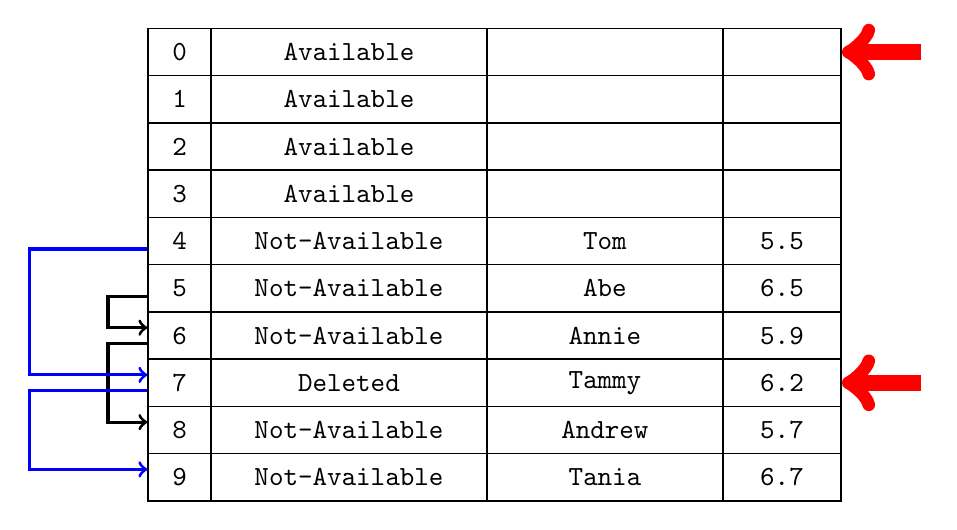
\begin{tikzpicture}

\draw (1.4, 0.7)
  node[draw, line width=0.02cm, , color=black,
       rounded corners=0cm, inner sep=0cm] {

\begin{minipage}[t][0.6cm]{0.8cm}
\mbox{}

\end{minipage}

};\draw (1.4, 0.7) node[color=black] {{\texttt{0}}};
\draw (3.55, 0.7)
  node[draw, line width=0.02cm, , color=black,
       rounded corners=0cm, inner sep=0cm] {

\begin{minipage}[t][0.6cm]{3.5cm}
\mbox{}

\end{minipage}

};\draw (3.55, 0.7) node[color=black] {{\texttt{Available}}};
\draw (6.800000000000001, 0.7)
  node[draw, line width=0.02cm, , color=black,
       rounded corners=0cm, inner sep=0cm] {

\begin{minipage}[t][0.6cm]{3.0cm}
\mbox{}

\end{minipage}

};\draw (6.800000000000001, 0.7) node[color=black] {{\texttt{}}};
\draw (9.05, 0.7)
  node[draw, line width=0.02cm, , color=black,
       rounded corners=0cm, inner sep=0cm] {

\begin{minipage}[t][0.6cm]{1.5cm}
\mbox{}

\end{minipage}

};\draw (9.05, 0.7) node[color=black] {{\texttt{}}};
\draw (1.4, 0.09999999999999987)
  node[draw, line width=0.02cm, , color=black,
       rounded corners=0cm, inner sep=0cm] {

\begin{minipage}[t][0.6cm]{0.8cm}
\mbox{}

\end{minipage}

};\draw (1.4, 0.09999999999999987) node[color=black] {{\texttt{1}}};
\draw (3.55, 0.09999999999999987)
  node[draw, line width=0.02cm, , color=black,
       rounded corners=0cm, inner sep=0cm] {

\begin{minipage}[t][0.6cm]{3.5cm}
\mbox{}

\end{minipage}

};\draw (3.55, 0.09999999999999987) node[color=black] {{\texttt{Available}}};
\draw (6.800000000000001, 0.09999999999999987)
  node[draw, line width=0.02cm, , color=black,
       rounded corners=0cm, inner sep=0cm] {

\begin{minipage}[t][0.6cm]{3.0cm}
\mbox{}

\end{minipage}

};\draw (6.800000000000001, 0.09999999999999987) node[color=black] {{\texttt{}}};
\draw (9.05, 0.09999999999999987)
  node[draw, line width=0.02cm, , color=black,
       rounded corners=0cm, inner sep=0cm] {

\begin{minipage}[t][0.6cm]{1.5cm}
\mbox{}

\end{minipage}

};\draw (9.05, 0.09999999999999987) node[color=black] {{\texttt{}}};
\draw (1.4, -0.5000000000000002)
  node[draw, line width=0.02cm, , color=black,
       rounded corners=0cm, inner sep=0cm] {

\begin{minipage}[t][0.6cm]{0.8cm}
\mbox{}

\end{minipage}

};\draw (1.4, -0.5000000000000002) node[color=black] {{\texttt{2}}};
\draw (3.55, -0.5000000000000002)
  node[draw, line width=0.02cm, , color=black,
       rounded corners=0cm, inner sep=0cm] {

\begin{minipage}[t][0.6cm]{3.5cm}
\mbox{}

\end{minipage}

};\draw (3.55, -0.5000000000000002) node[color=black] {{\texttt{Available}}};
\draw (6.800000000000001, -0.5000000000000002)
  node[draw, line width=0.02cm, , color=black,
       rounded corners=0cm, inner sep=0cm] {

\begin{minipage}[t][0.6cm]{3.0cm}
\mbox{}

\end{minipage}

};\draw (6.800000000000001, -0.5000000000000002) node[color=black] {{\texttt{}}};
\draw (9.05, -0.5000000000000002)
  node[draw, line width=0.02cm, , color=black,
       rounded corners=0cm, inner sep=0cm] {

\begin{minipage}[t][0.6cm]{1.5cm}
\mbox{}

\end{minipage}

};\draw (9.05, -0.5000000000000002) node[color=black] {{\texttt{}}};
\draw (1.4, -1.1000000000000003)
  node[draw, line width=0.02cm, , color=black,
       rounded corners=0cm, inner sep=0cm] {

\begin{minipage}[t][0.6cm]{0.8cm}
\mbox{}

\end{minipage}

};\draw (1.4, -1.1000000000000003) node[color=black] {{\texttt{3}}};
\draw (3.55, -1.1000000000000003)
  node[draw, line width=0.02cm, , color=black,
       rounded corners=0cm, inner sep=0cm] {

\begin{minipage}[t][0.6cm]{3.5cm}
\mbox{}

\end{minipage}

};\draw (3.55, -1.1000000000000003) node[color=black] {{\texttt{Available}}};
\draw (6.800000000000001, -1.1000000000000003)
  node[draw, line width=0.02cm, , color=black,
       rounded corners=0cm, inner sep=0cm] {

\begin{minipage}[t][0.6cm]{3.0cm}
\mbox{}

\end{minipage}

};\draw (6.800000000000001, -1.1000000000000003) node[color=black] {{\texttt{}}};
\draw (9.05, -1.1000000000000003)
  node[draw, line width=0.02cm, , color=black,
       rounded corners=0cm, inner sep=0cm] {

\begin{minipage}[t][0.6cm]{1.5cm}
\mbox{}

\end{minipage}

};\draw (9.05, -1.1000000000000003) node[color=black] {{\texttt{}}};
\draw (1.4, -1.7000000000000002)
  node[draw, line width=0.02cm, , color=black,
       rounded corners=0cm, inner sep=0cm] {

\begin{minipage}[t][0.6cm]{0.8cm}
\mbox{}

\end{minipage}

};\draw (1.4, -1.7000000000000002) node[color=black] {{\texttt{4}}};
\draw (3.55, -1.7000000000000002)
  node[draw, line width=0.02cm, , color=black,
       rounded corners=0cm, inner sep=0cm] {

\begin{minipage}[t][0.6cm]{3.5cm}
\mbox{}

\end{minipage}

};\draw (3.55, -1.7000000000000002) node[color=black] {{\texttt{Not-Available}}};
\draw (6.800000000000001, -1.7000000000000002)
  node[draw, line width=0.02cm, , color=black,
       rounded corners=0cm, inner sep=0cm] {

\begin{minipage}[t][0.6cm]{3.0cm}
\mbox{}

\end{minipage}

};\draw (6.800000000000001, -1.7000000000000002) node[color=black] {{\texttt{Tom}}};
\draw (9.05, -1.7000000000000002)
  node[draw, line width=0.02cm, , color=black,
       rounded corners=0cm, inner sep=0cm] {

\begin{minipage}[t][0.6cm]{1.5cm}
\mbox{}

\end{minipage}

};\draw (9.05, -1.7000000000000002) node[color=black] {{\texttt{5.5}}};
\draw (1.4, -2.3000000000000003)
  node[draw, line width=0.02cm, , color=black,
       rounded corners=0cm, inner sep=0cm] {

\begin{minipage}[t][0.6cm]{0.8cm}
\mbox{}

\end{minipage}

};\draw (1.4, -2.3000000000000003) node[color=black] {{\texttt{5}}};
\draw (3.55, -2.3000000000000003)
  node[draw, line width=0.02cm, , color=black,
       rounded corners=0cm, inner sep=0cm] {

\begin{minipage}[t][0.6cm]{3.5cm}
\mbox{}

\end{minipage}

};\draw (3.55, -2.3000000000000003) node[color=black] {{\texttt{Not-Available}}};
\draw (6.800000000000001, -2.3000000000000003)
  node[draw, line width=0.02cm, , color=black,
       rounded corners=0cm, inner sep=0cm] {

\begin{minipage}[t][0.6cm]{3.0cm}
\mbox{}

\end{minipage}

};\draw (6.800000000000001, -2.3000000000000003) node[color=black] {{\texttt{Abe}}};
\draw (9.05, -2.3000000000000003)
  node[draw, line width=0.02cm, , color=black,
       rounded corners=0cm, inner sep=0cm] {

\begin{minipage}[t][0.6cm]{1.5cm}
\mbox{}

\end{minipage}

};\draw (9.05, -2.3000000000000003) node[color=black] {{\texttt{6.5}}};
\draw (1.4, -2.9000000000000004)
  node[draw, line width=0.02cm, , color=black,
       rounded corners=0cm, inner sep=0cm] {

\begin{minipage}[t][0.6cm]{0.8cm}
\mbox{}

\end{minipage}

};\draw (1.4, -2.9000000000000004) node[color=black] {{\texttt{6}}};
\draw (3.55, -2.9000000000000004)
  node[draw, line width=0.02cm, , color=black,
       rounded corners=0cm, inner sep=0cm] {

\begin{minipage}[t][0.6cm]{3.5cm}
\mbox{}

\end{minipage}

};\draw (3.55, -2.9000000000000004) node[color=black] {{\texttt{Not-Available}}};
\draw (6.800000000000001, -2.9000000000000004)
  node[draw, line width=0.02cm, , color=black,
       rounded corners=0cm, inner sep=0cm] {

\begin{minipage}[t][0.6cm]{3.0cm}
\mbox{}

\end{minipage}

};\draw (6.800000000000001, -2.9000000000000004) node[color=black] {{\texttt{Annie}}};
\draw (9.05, -2.9000000000000004)
  node[draw, line width=0.02cm, , color=black,
       rounded corners=0cm, inner sep=0cm] {

\begin{minipage}[t][0.6cm]{1.5cm}
\mbox{}

\end{minipage}

};\draw (9.05, -2.9000000000000004) node[color=black] {{\texttt{5.9}}};
\draw (1.4, -3.500000000000001)
  node[draw, line width=0.02cm, , color=black,
       rounded corners=0cm, inner sep=0cm] {

\begin{minipage}[t][0.6cm]{0.8cm}
\mbox{}

\end{minipage}

};\draw (1.4, -3.500000000000001) node[color=black] {{\texttt{7}}};
\draw (3.55, -3.500000000000001)
  node[draw, line width=0.02cm, , color=black,
       rounded corners=0cm, inner sep=0cm] {

\begin{minipage}[t][0.6cm]{3.5cm}
\mbox{}

\end{minipage}

};\draw (3.55, -3.500000000000001) node[color=black] {{\texttt{Deleted}}};
\draw (6.800000000000001, -3.500000000000001)
  node[draw, line width=0.02cm, , color=black,
       rounded corners=0cm, inner sep=0cm] {

\begin{minipage}[t][0.6cm]{3.0cm}
\mbox{}

\end{minipage}

};\draw (6.800000000000001, -3.500000000000001) node[color=black] {{\texttt{Tammy}}};
\draw (9.05, -3.500000000000001)
  node[draw, line width=0.02cm, , color=black,
       rounded corners=0cm, inner sep=0cm] {

\begin{minipage}[t][0.6cm]{1.5cm}
\mbox{}

\end{minipage}

};\draw (9.05, -3.500000000000001) node[color=black] {{\texttt{6.2}}};
\draw (1.4, -4.1000000000000005)
  node[draw, line width=0.02cm, , color=black,
       rounded corners=0cm, inner sep=0cm] {

\begin{minipage}[t][0.6cm]{0.8cm}
\mbox{}

\end{minipage}

};\draw (1.4, -4.1000000000000005) node[color=black] {{\texttt{8}}};
\draw (3.55, -4.1000000000000005)
  node[draw, line width=0.02cm, , color=black,
       rounded corners=0cm, inner sep=0cm] {

\begin{minipage}[t][0.6cm]{3.5cm}
\mbox{}

\end{minipage}

};\draw (3.55, -4.1000000000000005) node[color=black] {{\texttt{Not-Available}}};
\draw (6.800000000000001, -4.1000000000000005)
  node[draw, line width=0.02cm, , color=black,
       rounded corners=0cm, inner sep=0cm] {

\begin{minipage}[t][0.6cm]{3.0cm}
\mbox{}

\end{minipage}

};\draw (6.800000000000001, -4.1000000000000005) node[color=black] {{\texttt{Andrew}}};
\draw (9.05, -4.1000000000000005)
  node[draw, line width=0.02cm, , color=black,
       rounded corners=0cm, inner sep=0cm] {

\begin{minipage}[t][0.6cm]{1.5cm}
\mbox{}

\end{minipage}

};\draw (9.05, -4.1000000000000005) node[color=black] {{\texttt{5.7}}};
\draw (1.4, -4.7)
  node[draw, line width=0.02cm, , color=black,
       rounded corners=0cm, inner sep=0cm] {

\begin{minipage}[t][0.6cm]{0.8cm}
\mbox{}

\end{minipage}

};\draw (1.4, -4.7) node[color=black] {{\texttt{9}}};
\draw (3.55, -4.7)
  node[draw, line width=0.02cm, , color=black,
       rounded corners=0cm, inner sep=0cm] {

\begin{minipage}[t][0.6cm]{3.5cm}
\mbox{}

\end{minipage}

};\draw (3.55, -4.7) node[color=black] {{\texttt{Not-Available}}};
\draw (6.800000000000001, -4.7)
  node[draw, line width=0.02cm, , color=black,
       rounded corners=0cm, inner sep=0cm] {

\begin{minipage}[t][0.6cm]{3.0cm}
\mbox{}

\end{minipage}

};\draw (6.800000000000001, -4.7) node[color=black] {{\texttt{Tania}}};
\draw (9.05, -4.7)
  node[draw, line width=0.02cm, , color=black,
       rounded corners=0cm, inner sep=0cm] {

\begin{minipage}[t][0.6cm]{1.5cm}
\mbox{}

\end{minipage}

};\draw (9.05, -4.7) node[color=black] {{\texttt{6.7}}};\draw[line width=0.04cm,black,->] (0.99,-2.4) to  (0.49,-2.4) to  (0.49,-2.8) to  (0.99,-2.8);
\draw[line width=0.04cm,black,->] (0.99,-3.0) to  (0.49,-3.0) to  (0.49,-4.0) to  (0.99,-4.0);
\draw[line width=0.04cm,blue,->] (0.99,-1.8) to  (-0.51,-1.8) to  (-0.51,-3.4) to  (0.99,-3.4);
\draw[line width=0.04cm,blue,->] (0.99,-3.6) to  (-0.51,-3.6) to  (-0.51,-4.6) to  (0.99,-4.6);
\draw[line width=0.2cm,red,->] (10.81,-3.5) to  (9.81,-3.5);
\draw[line width=0.2cm,red,->] (10.81,0.7) to  (9.81,0.7);
\end{tikzpicture}

\end{center}



I then compare \verb!9! and \verb!5! and decide to swap again to get:

\begin{center}
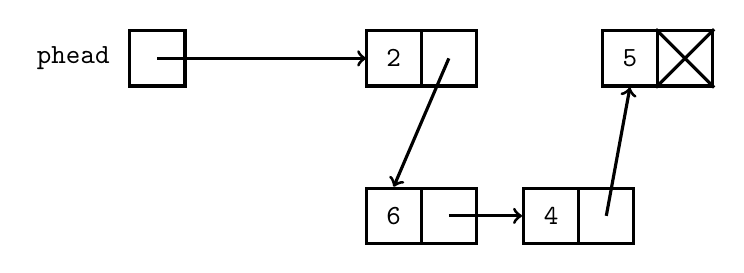
\begin{tikzpicture}

\draw (0.35, 0.35)
  node[draw, line width=0.04cm, , color=black,
       rounded corners=0cm, inner sep=0cm] {

\begin{minipage}[t][0.7cm]{0.7cm}
\mbox{}

\end{minipage}

};\draw (0.35, 0.35) node[color=black] {{\texttt{2}}};
\draw (1.0499999999999998, 0.35)
  node[draw, line width=0.04cm, , color=black,
       rounded corners=0cm, inner sep=0cm] {

\begin{minipage}[t][0.7cm]{0.7cm}
\mbox{}

\end{minipage}

};\draw (1.0499999999999998, 0.35) node[color=black] {{\texttt{}}};
\draw (0.35, -1.65)
  node[draw, line width=0.04cm, , color=black,
       rounded corners=0cm, inner sep=0cm] {

\begin{minipage}[t][0.7cm]{0.7cm}
\mbox{}

\end{minipage}

};\draw (0.35, -1.65) node[color=black] {{\texttt{6}}};
\draw (1.0499999999999998, -1.65)
  node[draw, line width=0.04cm, , color=black,
       rounded corners=0cm, inner sep=0cm] {

\begin{minipage}[t][0.7cm]{0.7cm}
\mbox{}

\end{minipage}

};\draw (1.0499999999999998, -1.65) node[color=black] {{\texttt{}}};
\draw (2.35, -1.65)
  node[draw, line width=0.04cm, , color=black,
       rounded corners=0cm, inner sep=0cm] {

\begin{minipage}[t][0.7cm]{0.7cm}
\mbox{}

\end{minipage}

};\draw (2.35, -1.65) node[color=black] {{\texttt{4}}};
\draw (3.0500000000000003, -1.65)
  node[draw, line width=0.04cm, , color=black,
       rounded corners=0cm, inner sep=0cm] {

\begin{minipage}[t][0.7cm]{0.7cm}
\mbox{}

\end{minipage}

};\draw (3.0500000000000003, -1.65) node[color=black] {{\texttt{}}};
\draw (3.35, 0.35)
  node[draw, line width=0.04cm, , color=black,
       rounded corners=0cm, inner sep=0cm] {

\begin{minipage}[t][0.7cm]{0.7cm}
\mbox{}

\end{minipage}

};\draw (3.35, 0.35) node[color=black] {{\texttt{5}}};
\draw (4.05, 0.35)
  node[draw, line width=0.04cm, , color=black,
       rounded corners=0cm, inner sep=0cm] {

\begin{minipage}[t][0.7cm]{0.7cm}
\mbox{}

\end{minipage}

};\draw (4.05, 0.35) node[color=black] {{\texttt{}}};\draw[line width=0.04cm,black,->] (1.05,0.35) to  (0.35,-1.28);
\draw[line width=0.04cm,black,->] (1.05,-1.65) to  (1.98,-1.65);
\draw[line width=0.04cm,black,->] (3.05,-1.65) to  (3.35,-0.02);
\draw[line width=0.04cm,black] (3.68,0.72) to  (4.42,-0.02);
\draw[line width=0.04cm,black] (4.42,0.72) to  (3.68,-0.02);

\draw (-2.65, 0.35)
  node[draw, line width=0.04cm, , color=black,
       rounded corners=0cm, inner sep=0cm] {

\begin{minipage}[t][0.7cm]{0.7cm}
\mbox{}

\end{minipage}

};\draw (-2.65, 0.35) node[color=black] {{\texttt{}}};\draw[line width=0.04cm,black,->] (-2.65,0.35) to  (0,0.35);

\draw (-3.7199999999999998, 0.35)
  node[draw, line width=0.04cm, , color=white,
       rounded corners=0cm, inner sep=0cm] {

\begin{minipage}[t][0.1cm]{0.1cm}
\mbox{}

\end{minipage}

};\draw (-3.7199999999999998, 0.35) node[color=black] {{\texttt{phead}}};
\end{tikzpicture}

\end{center}



Now it's a maxheap.
Basically, you continually swap the value in question with
its parent if the value is larger than the parent.

This is called
\defone{heapify-up}.
It's also called
\defone{bubble up} or
\defone{percolate up}.


In general, if \verb!x[0..n]! is an array
and I can talk about heapify-up on array \verb!x!
treating \verb!x! as a maxheap,
starting at index \verb!i! and going up
along its path to the root (i.e., index 0).

You can also talk about heapify-up on an array
treating it as a minheap,
starting at some index.

For a maxheap, to heapify-up at an index \verb!i!, you compare
\verb!x[i]! and \verb!x[parent(i)]!
and swap them if necessary, i.e. if \verb!x[i]! $>$ \verb!x[parent(i)]!
and you keep following that value up to the root.
If \verb!x[i]! $\leq$ \verb!x[parent(i)]!, you stop.
That's it.

\begin{Verbatim}[frame=single]
ALGORITHM: heapify-up (for maxheap)
INPUTS: x[0..n-1] -- array
        i         -- index of x

while 1:
    if parent(i) < 0: break
    if x[i] > x[parent(i)]:
        swap x[i], x[parent(i)]
        i = parent(i)
\end{Verbatim}

With a tiny of optimization:
\begin{Verbatim}[frame=single]
ALGORITHM: heapify-up (for maxheap)
INPUTS: x[0..n-1] -- array
        i         -- index of x

v = x[i]
while 1:
    p = parent(i)
    if p < 0: break
    if v <= x[p]:
        x[i] = v
        break
    else:
        x[i] = x[p]
        i = p
\end{Verbatim}

The same idea works for minheap.
